\documentclass[xcolor=table, 11pt, aspectratio=169]{beamer}

%\usepackage{arev}
\usepackage{amsmath,amssymb,amscd}
\usepackage{dsfont}
\usepackage{mathrsfs}
\usepackage{yfonts}
\usepackage{bm}
\usepackage{graphicx}
\usepackage{tabularx}
\usepackage{animate}
\usepackage{listings}
\usepackage{pifont}
%\usepackage{mathtools}
%\usepackage{ifthen}

%\usepackage{xeCJK}
%\usepackage{fontspec}
%\newfontfamily\cjkfont{PingFang SC}
%\setCJKmainfont{PingFang SC}
\newcolumntype{x}{>{\centering\arraybackslash}X}
\renewcommand{\arraystretch}{1.5}
\newcommand{\uone}{\mathrm U(1)}
\DeclareMathOperator{\img}{img}
\lstset{language=GAP}

\usepackage{tikz}
	\usetikzlibrary{calc}
	\usetikzlibrary{arrows,shapes, positioning, matrix}
	\usetikzlibrary{decorations.markings}
	\tikzset{>=stealth}
	\tikzstyle arrowstyle=[scale=1]
	\tikzstyle directed=[postaction={decorate,decoration={markings,
 	   mark=at position .15 with {\arrow[arrowstyle]{stealth}}}}]
\tikzstyle string=[thick,postaction={decorate,decoration={markings,
    mark=at position .55 with {\arrow[arrowstyle]{stealth}}}}]
\tikzstyle dual_string=[dashed,postaction={decorate,decoration={markings,
    mark=at position .55 with {\arrow[arrowstyle]{stealth}}}}]

\tikzstyle dw=[thick,postaction={decorate,decoration={markings,
    mark=at position 1 with {\arrow[arrowstyle]{stealth}}}}]
\tikzstyle group=[mbg]
\newcommand*{\halfway}{0.5*\pgfdecoratedpathlength+.5*8pt}\tikzstyle arrowstyle=[scale=1]
\newcommand*{\halfwayb}{0.5*\pgfdecoratedpathlength}
\tikzstyle arrowstyle=[scale=1]
\tikzstyle fermion=[thick,postaction={decorate},decoration={markings,
    mark=at position \halfway with {\arrow[arrowstyle]{latex}}}]
\tikzstyle fermion2=[thick,postaction={decorate},decoration={markings,
        mark=at position \halfwayb with {\arrow[arrowstyle]{latex}}}]

\usepackage{pgffor}
\newcommand{\mb}[1]{\mathbf{#1}}
\renewcommand{\cal}[1]{\mathcal{#1}}

\newcommand{\ag}[2]{#1_\mb{#2}}
\newcommand{\cohosub}[1]{\scalebox{0.72}{\textswab{#1}}}
\newcommand{\cohosubsub}[1]{\scalebox{0.6}{\textswab{#1}}}
\newcommand{\coho}[1]{\textswab{#1}}

\DeclareMathOperator{\tr}{Tr}
\DeclareMathOperator{\im}{Im}
\DeclareMathOperator{\re}{Re}

\mode<presentation>
{
  %\usetheme{Warsaw}
  % or ...
  %\useoutertheme{rectangle}
  \setbeamertemplate{frametitle}[default][center]
  \defbeamertemplate{itemize item}{flat}{\begin{pgfpicture}{-1ex}{0ex}{1ex}{2ex}
      \pgfpathcircle{\pgfpoint{0pt}{.6ex}}{0.6ex}
      \pgfusepath{fill}
    \end{pgfpicture}%
  }
  \defbeamertemplate{itemize subitem}{flat}{\footnotesize\raise0.5pt\hbox{\textbullet}}
  \defbeamertemplate{itemize subsubitem}{flat}{\footnotesize\raise0.5pt\hbox{\textbullet}}

  %\useinnertheme{circles}
  \setbeamertemplate{items}[flat]
  \setbeamertemplate{sections/subsections in toc}[circle]
  \setbeamertemplate{blocks}[rounded]
  \setbeamertemplate{title page}[default][colsep=-4bp,rounded=true]
  \setbeamertemplate{part page}[default][colsep=-4bp,rounded=true]
  \setbeamercovered{transparent}
  %\usecolortheme{spruce}
  %\definecolor{THU}{RGB}{116,61,130}
  \definecolor{mbg}{RGB}{0,0,160}
  \setbeamercolor*{palette primary}{fg=white,bg=mbg}
  \setbeamercolor*{titlelike}{parent=palette primary}
  \setbeamercolor*{structure}{fg=mbg}
  \setbeamercolor{frametitle}{fg=white,bg=mbg}
  % or whatever (possibly just delete it)
  \setbeamercolor{block title}{bg=mbg,fg=white}
  \setbeamercolor{block body}{bg=mbg!15}


  \addtobeamertemplate{navigation symbols}{}{ \hspace{1em}%
    \usebeamerfont{footline}%
    \insertframenumber / \inserttotalframenumber }
}


%\usepackage[english]{babel}
% or whatever

%\usepackage[latin1]{inputenc}
% or whatever

%\usepackage{times}
%\usepackage[T1]{fontenc}
% Or whatever. Note that the encoding and the font should match. If T1
% does not look nice, try deleting the line with the fontenc.

\title[Space-group SPTs] % (optional, use only with long paper titles)
{Classification of topological crystalline states}

\author[Y Qi] % (optional, use only with lots of authors)
{Yang~Qi}
% - Give the names in the same order as the appear in the paper.
% - Use the \inst{?} command only if the authors have different
%   affiliation.

\institute[Fudan] % (optional, but mostly needed)
{Department of Physics, Fudan University}
% - Use the \inst command only if there are several affiliations.
% - Keep it simple, no one is interested in your street address.

%\date{2016 Annual Meeting of Fudan CFTPP} % (optional, should be abbreviation of conference name)
%{Fudan University, Oct 13 2015}
%\date{Hong Kong Forum of Physics, HKU, Jan 7-9, 2019.}
%\date{QuIST V, Kunming, Aug. 2nd, 2019.}
%\date{Perimeter Institute, Sept. 3rd, 2019.}
%\date{Beihang University, Oct. 22nd, 2019.}
%\date{QuIST VI, Chongqing, May 2021.}
\date{Fudan Annual Meeting, 2023}
% - Either use conference name or its abbreviation.
% - Not really informative to the audience, more for people (including
%   yourself) who are reading the slides online

\subject{Theoretical Physics}
% This is only inserted into the PDF information catalog. Can be left
% out.



% If you have a file called "university-logo-filename.xxx", where xxx
% is a graphic format that can be processed by latex or pdflatex,
% resp., then you can add a logo as follows:

\pgfdeclareimage[height=1cm]{university-logo}{../resources/fudan}
\logo{\pgfuseimage{university-logo}}

\AtBeginSection[]
{
\begin{frame}{Outline}
%	\begin{columns}
%		\begin{column}[t]{.45\textwidth}
%		\begin{center}
%			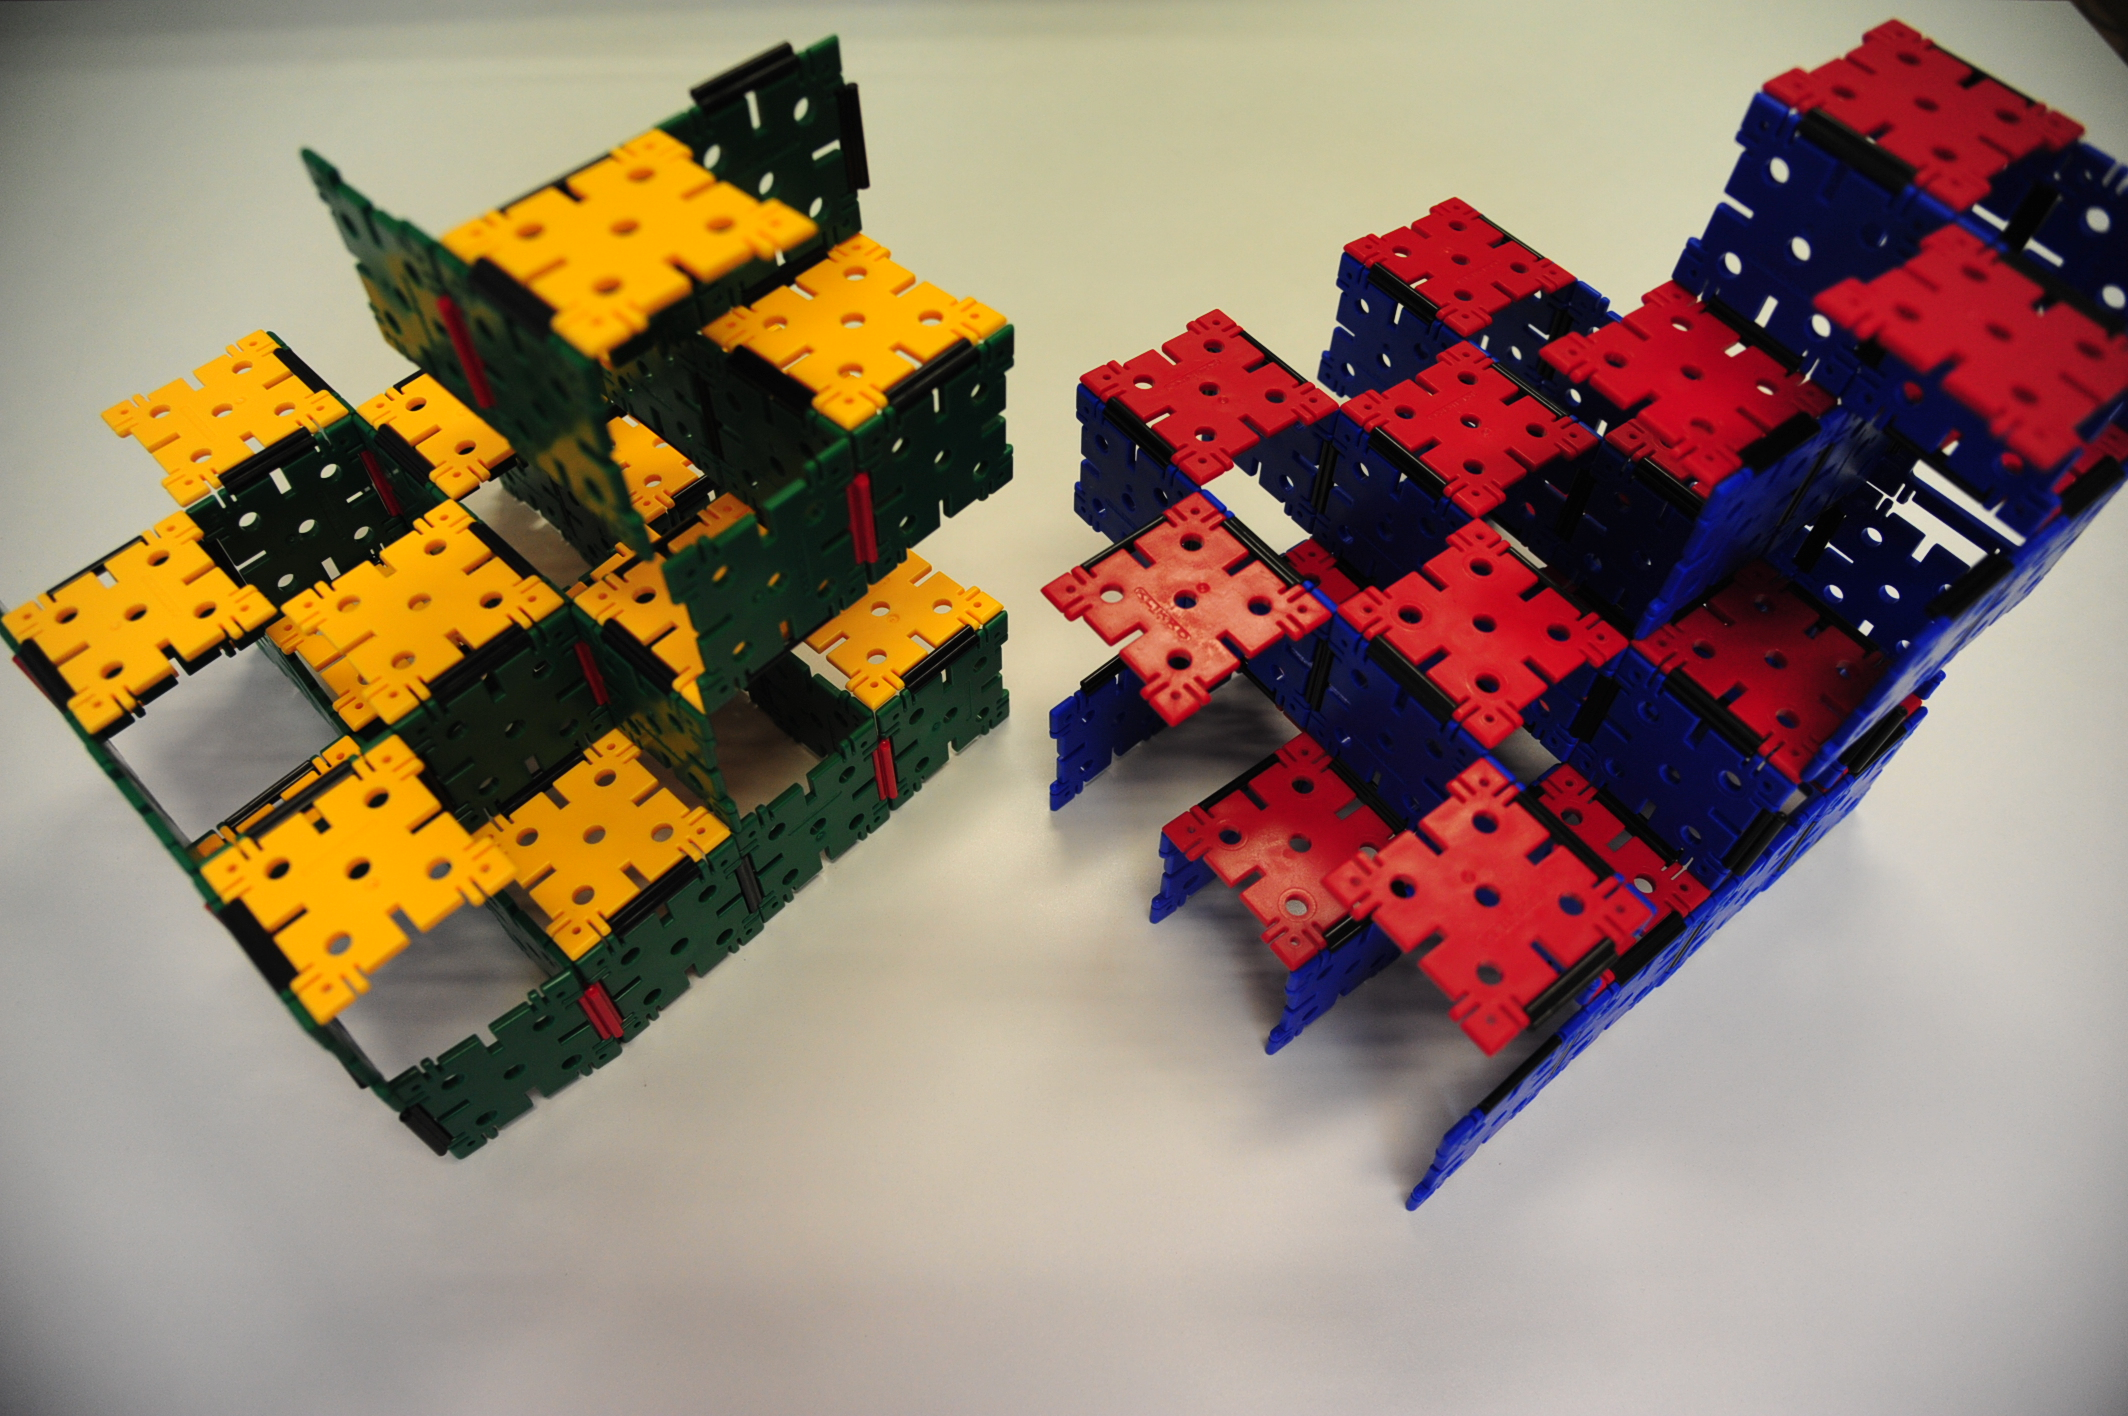
\includegraphics[height=4cm]{toys}
%		\end{center}
%	\end{column}
%	\begin{minipage}[t][0.5\textheight]{0.55\textwidth}
      \tableofcontents[currentsection]
%    \end{minipage}\hfill
%	\end{columns}
\end{frame}
}


% Delete this, if you do not want the table of contents to pop up at
% the beginning of each subsection:

\begin{document}

\begin{frame}
  \titlepage
\end{frame}

\begin{frame}{Collaborators}
  \begin{itemize}
  \item Yunqing Ouyang: Fudan University $\Rightarrow$ Huawei.
  \item Zhi-Da Song: Peking University.
  \item Qing-Rui Wang: Tsinghua University.
  \item Chen Fang: Institute of Physics, Beijing.
  \item Zheng-Cheng Gu: Chinese University of Hong Kong.
    \begin{center}
      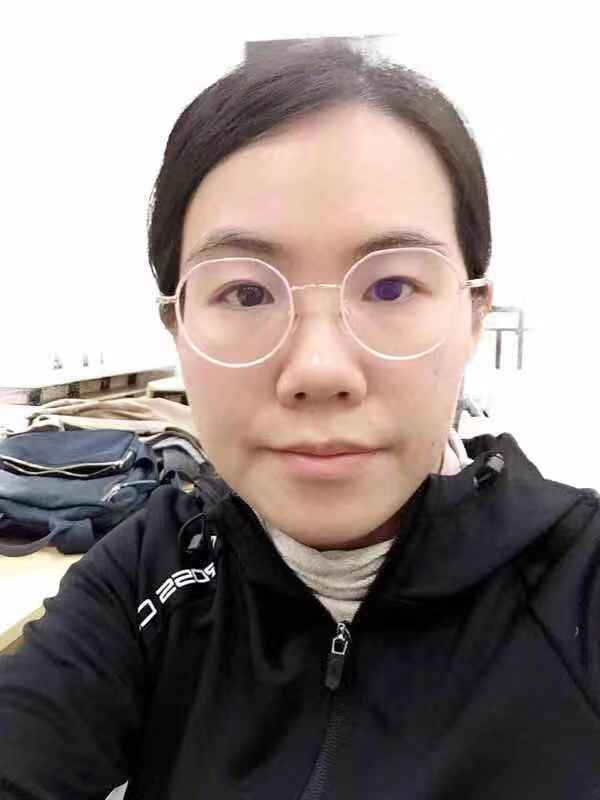
\includegraphics[height=2.5cm]{../people/yunqing}
      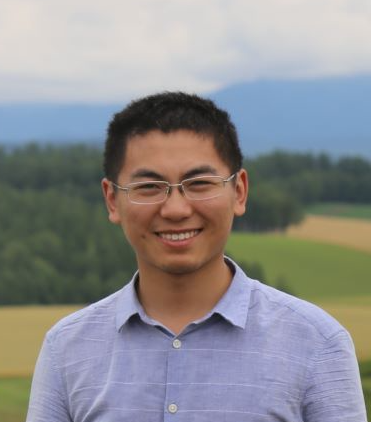
\includegraphics[height=2.5cm]{../people/zhidasong}
      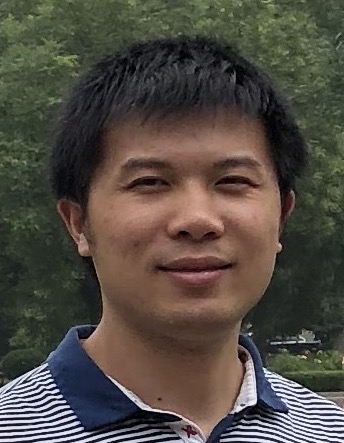
\includegraphics[height=2.5cm]{../people/qingrui}      
      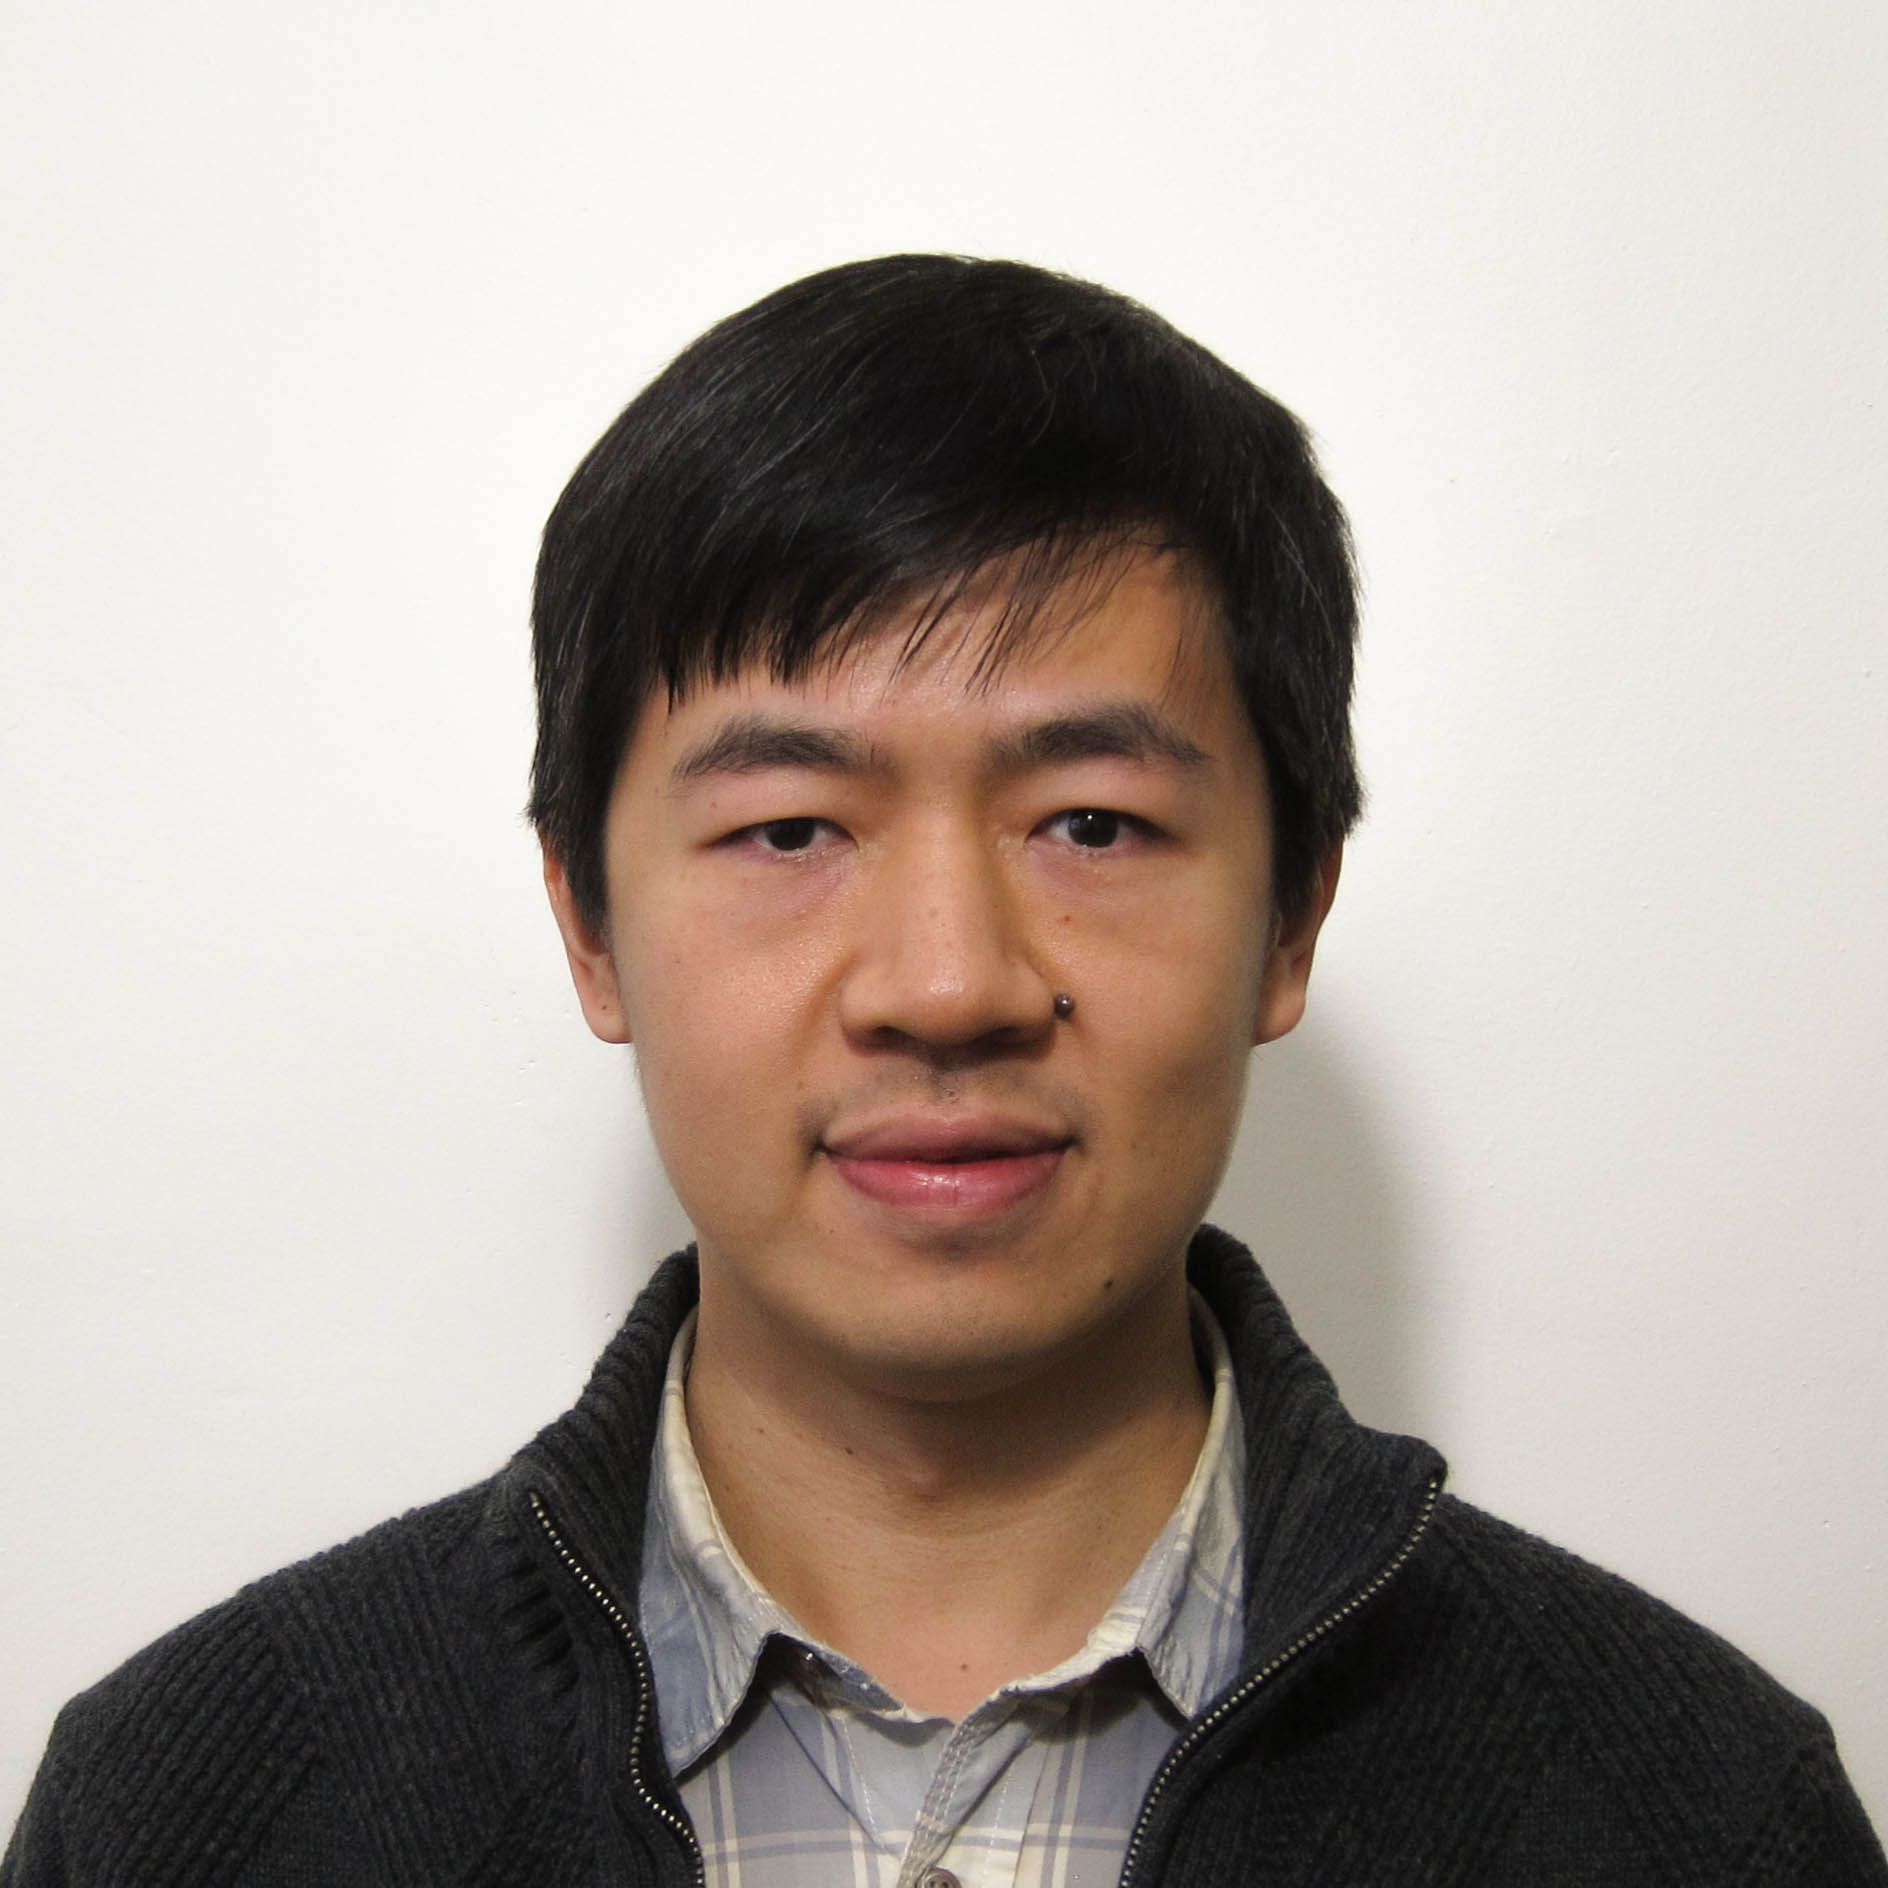
\includegraphics[height=2.5cm]{../people/chenfang}
      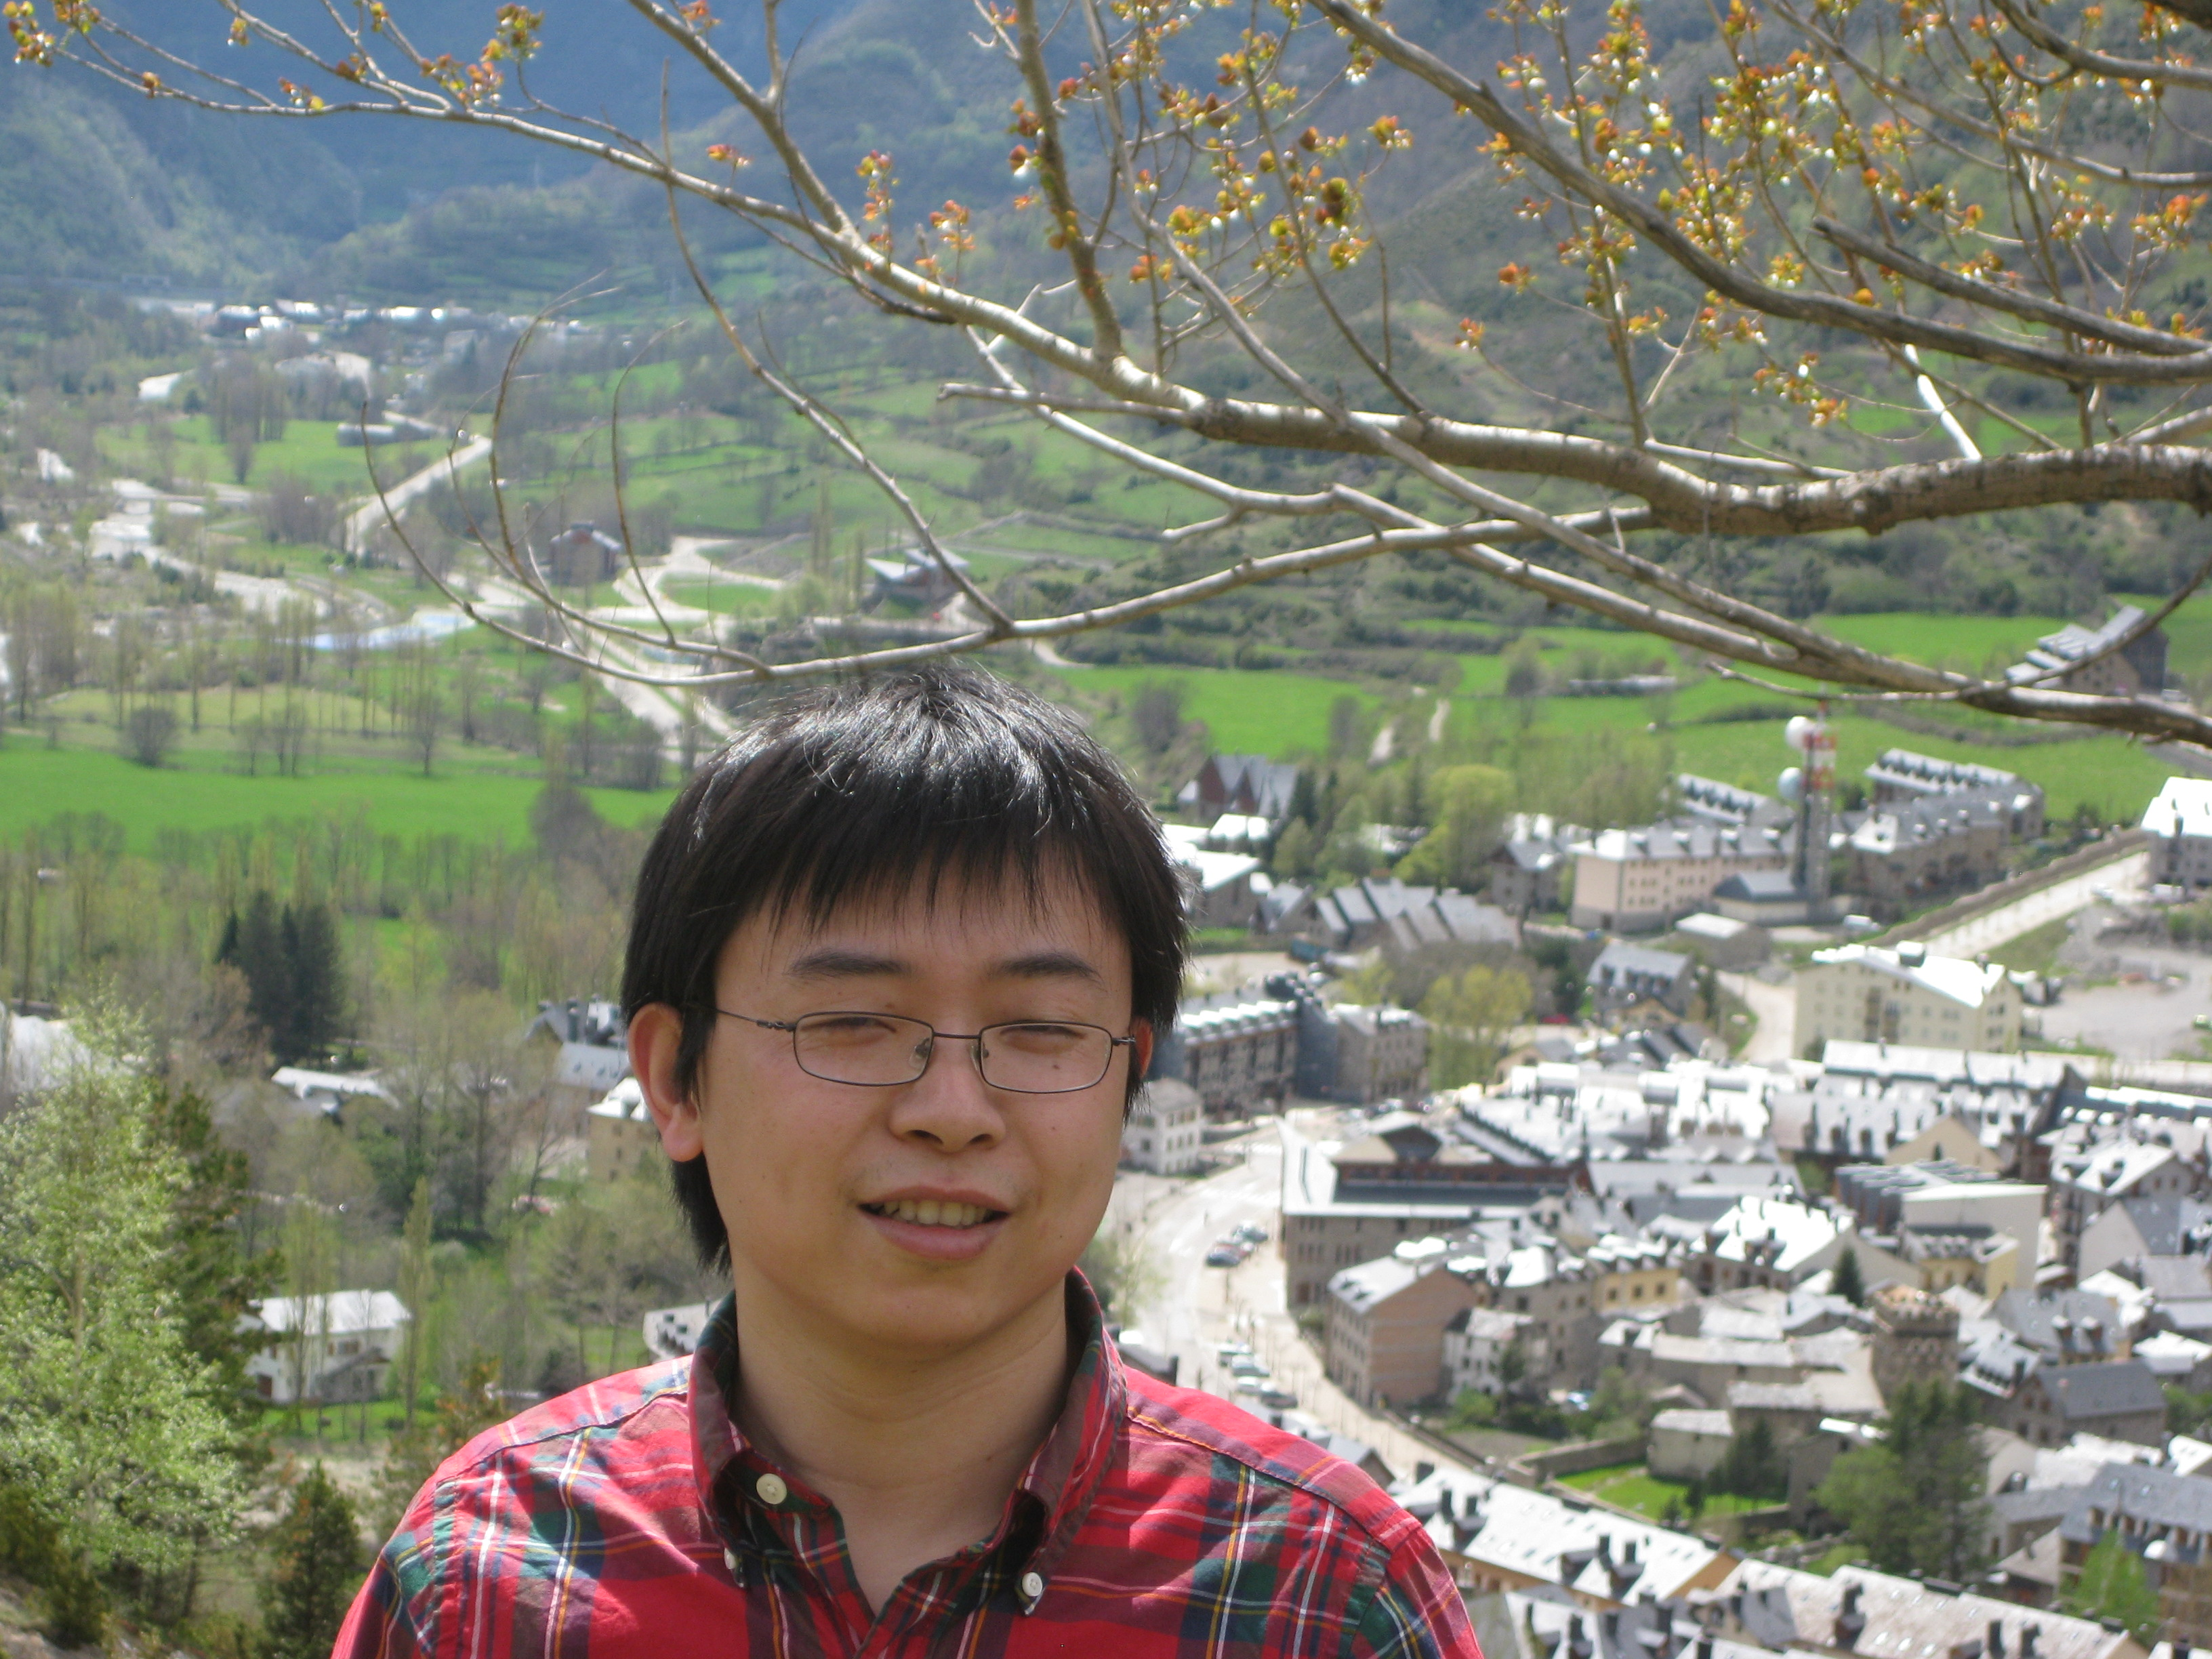
\includegraphics[height=2.5cm]{../people/zhengcheng}
    \end{center}
  \item Zhida Song, Chen Fang and YQ, Nature Communications \textbf{11} 4197 (2020).
  \item Yunqing Ouyang, Qing-Rui Wang, Zheng-Cheng Gu and YQ, Chin. Phys. Lett. \textbf{38} 127101 (2021).
\end{itemize}
\end{frame}

\begin{frame}{Outline}
%	\begin{columns}
%		\begin{column}[t]{.45\textwidth}
%		\begin{center}
%			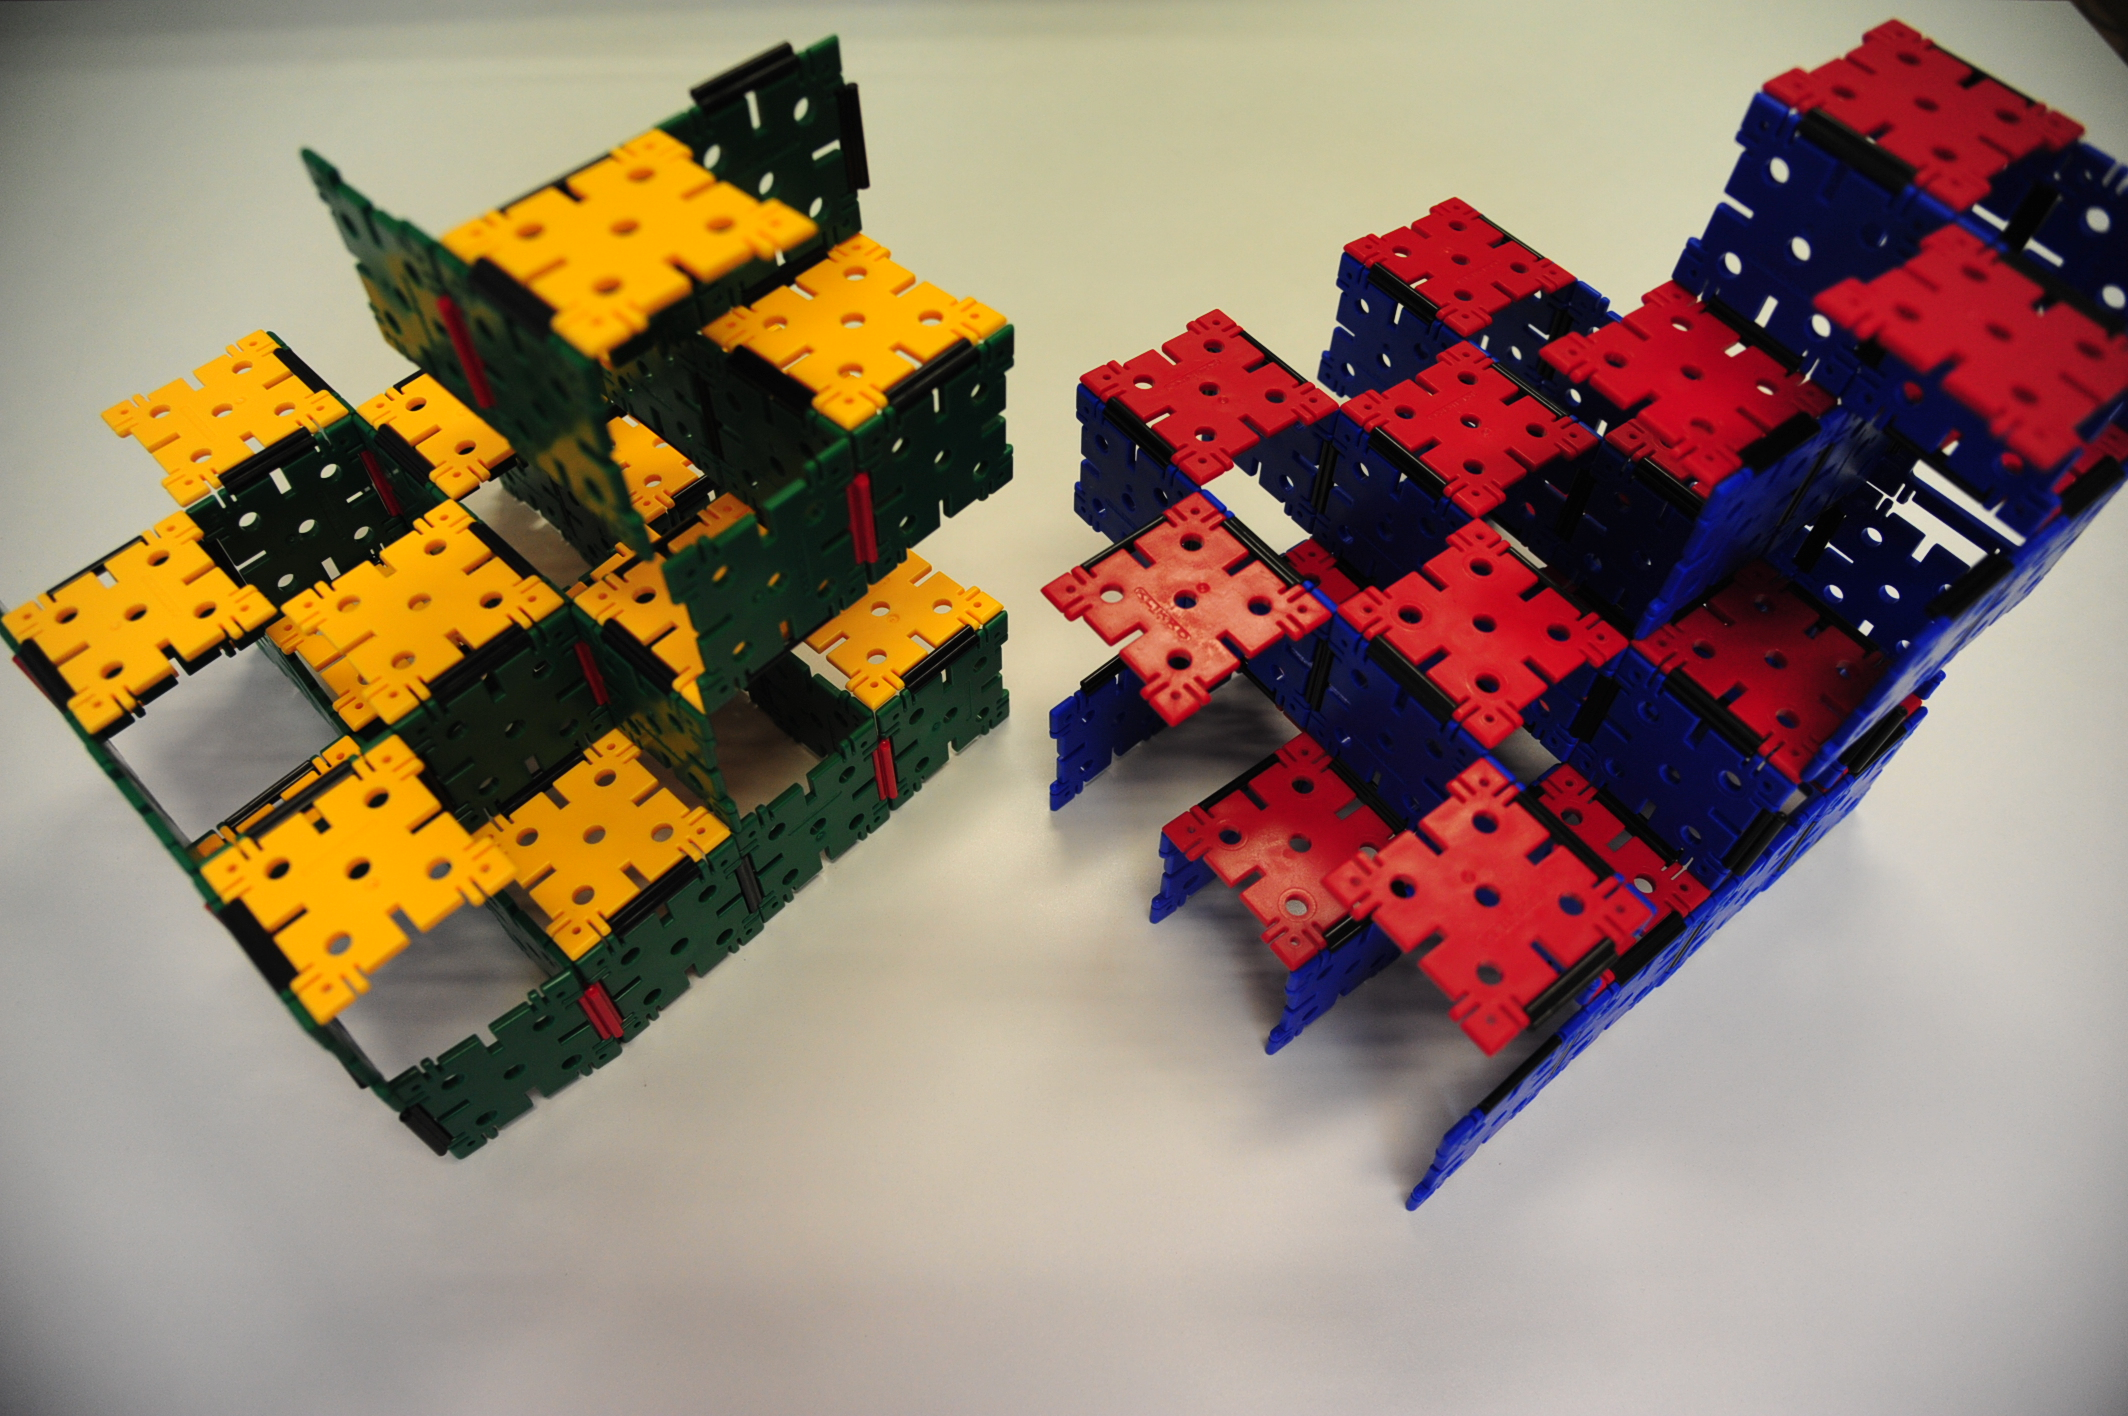
\includegraphics[height=4cm]{toys}
%		\end{center}
%	\end{column}
%	\begin{minipage}[t][0.5\textheight]{0.55\textwidth}
      \tableofcontents
%    \end{minipage}\hfill
%	\end{columns}
\end{frame}


\section{Introduction to SPT States}

\begin{frame}
  \frametitle{Symmetry-Protected Topological (SPT) states}
\begin{itemize}
\item SPT: gapped topological phases beyond Landau paradiam.
\item Gapped bulk : cannot be smoothly connected to a trivial state without closing gap or breaking symmetry.
\item Symmetry-protected gapless surface states.
\item Free-fermion states: topological insulators, topological superconductors: $K$-theory.
\item Bosonic SPTs: Haldane chain, CZX/Levin-Gu state, etc: Group Cohomology.
\item Interacting fermionic SPTs.
\end{itemize}
\end{frame}

\begin{frame}
  \frametitle{Abelian-group classification}
  \begin{itemize}
  \item SPT phases and boundary anomalies are classified by Abelian groups ($\mathbb Z$ or $\mathbb Z_n$).
    \begin{itemize}
    \item Addition: stacking of phases/gapless boundaries.
    \item 0: The trivial phase/gapped boundary.
    \end{itemize}
  \item Classification: determined by symmetry group $G$ and dimension $d$.
  \item 2D Chern-insulators (Integer Quantum Hall):
    \begin{center}
      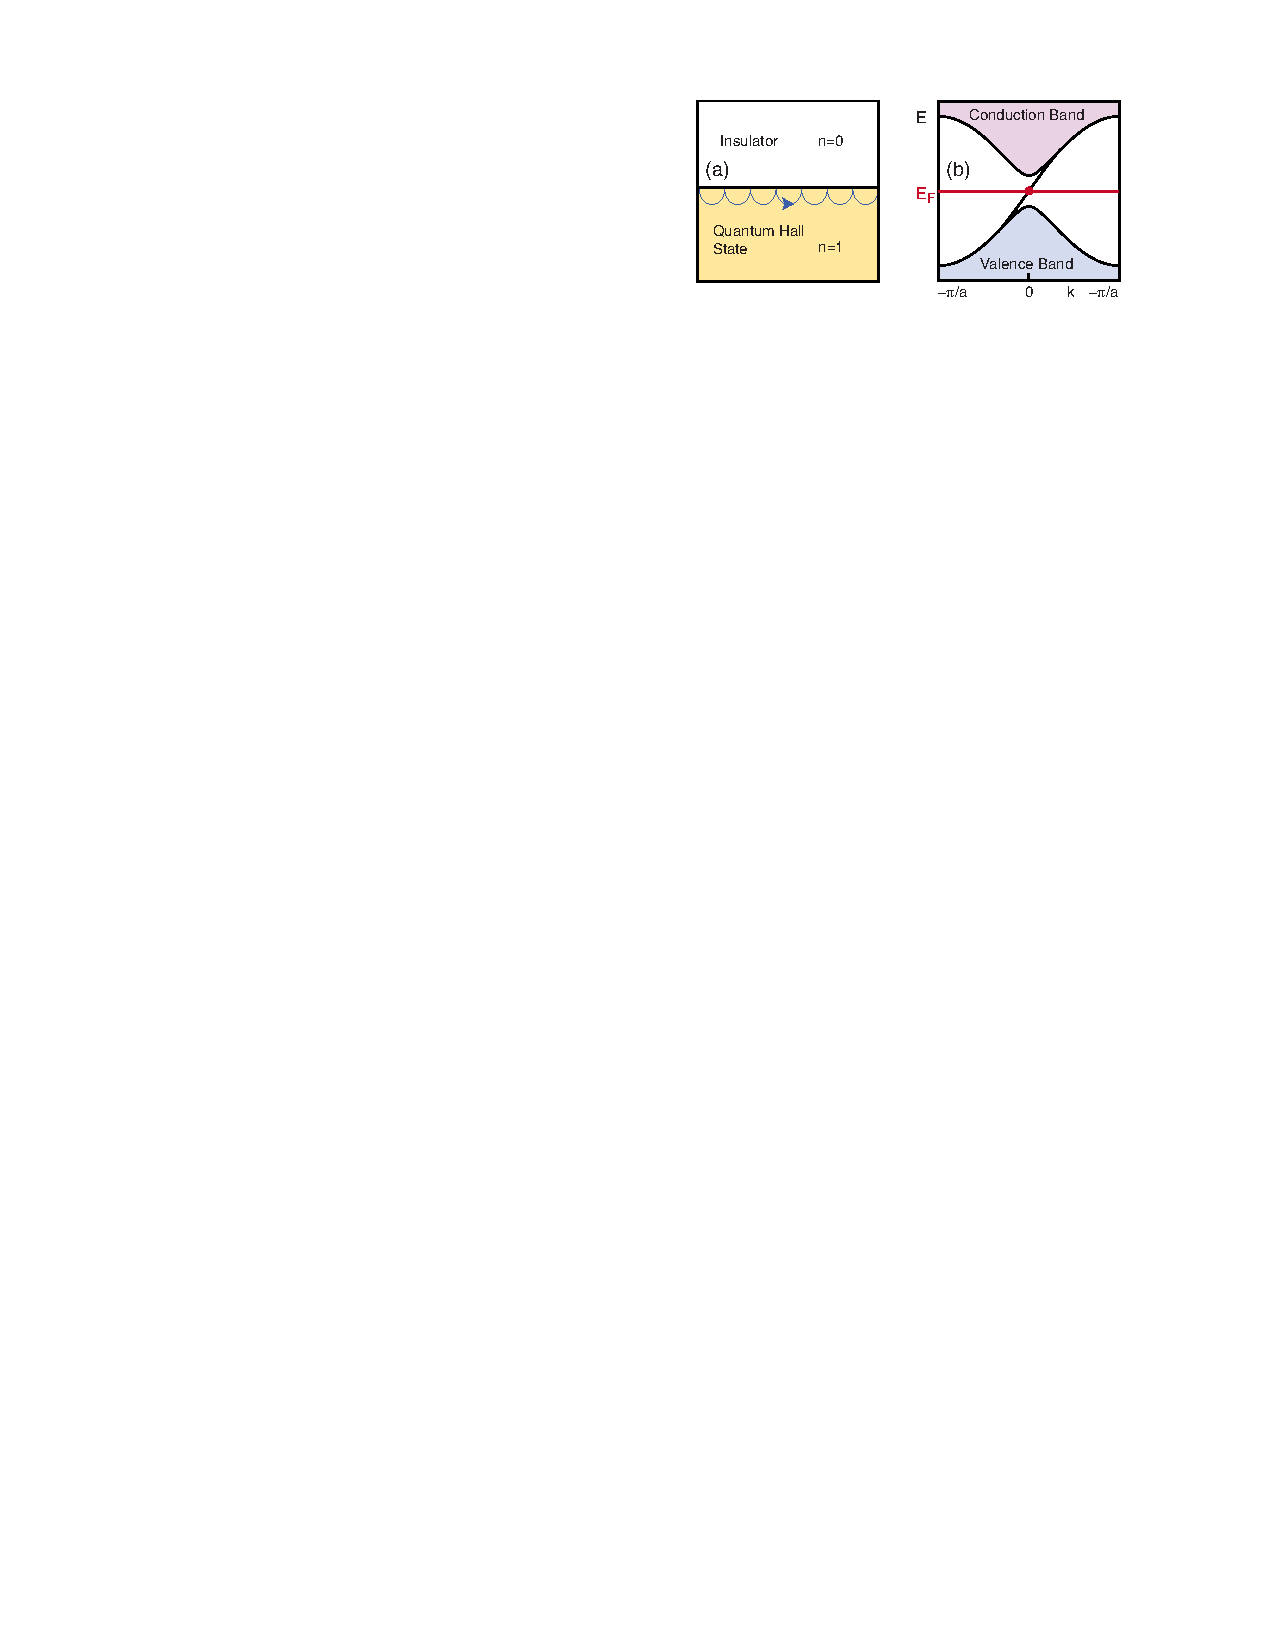
\includegraphics[width=8cm]{qhe_edge}
    \end{center}
    Classified by $\mathbb Z$: $[n]+[m]=[n+m]$; $[n]+[-n] = 0$.
  \end{itemize}
\end{frame}

\begin{frame}
	\frametitle{Abelian-group classification}
	\begin{itemize}
		\item 3D Topological Insulators:
		\begin{center}
			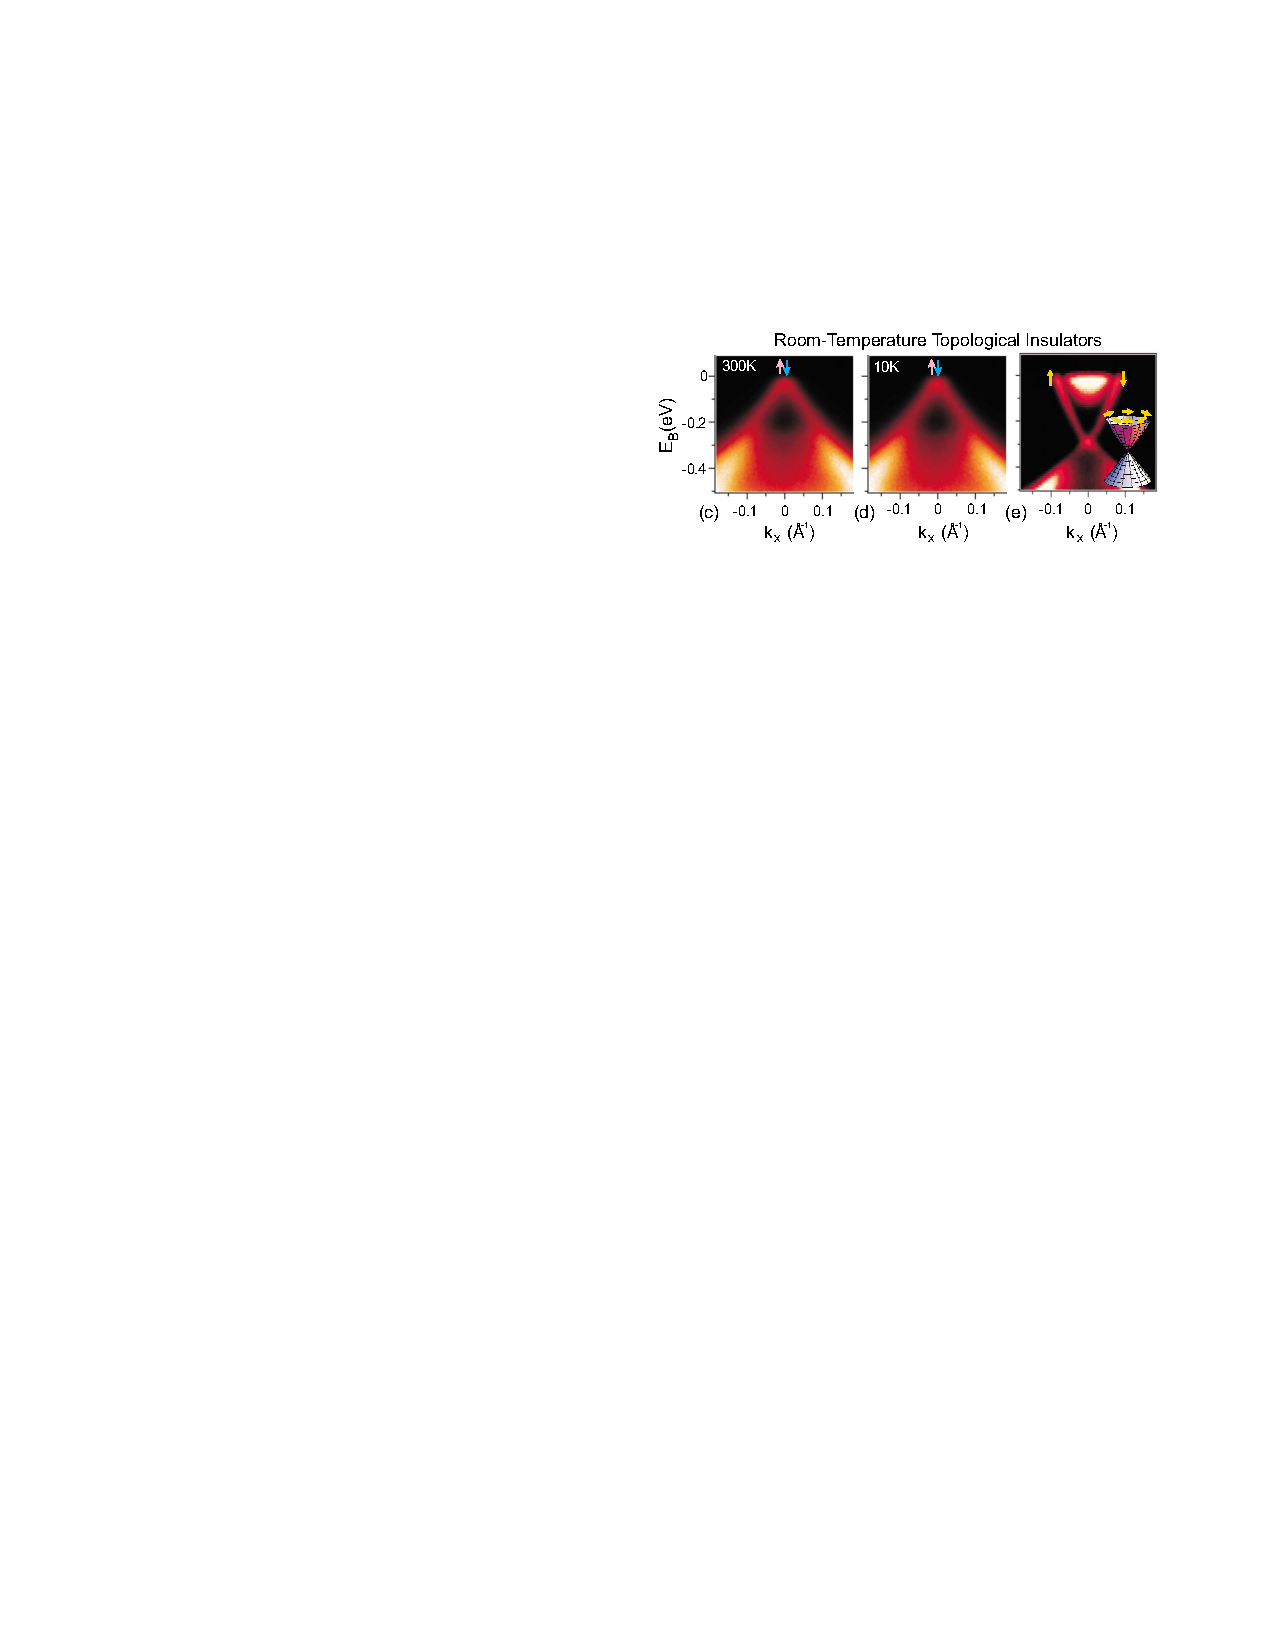
\includegraphics[width=8cm]{ti_surface}
		\end{center}
		Classified by $\mathbb Z_2$: $[1]+[1] = 0$.
		\item 1D Haldane chain:
		\begin{center}
			
\includegraphics[width=6cm]{../dimer/weak3d_aklt_blue}
		\end{center}
		Classified by $\mathbb Z_2$: $[1]+[1] = 0$.
	\end{itemize}
\end{frame}

\begin{frame}
\frametitle{Space-group SPT}
\begin{itemize}
\item Two approaches:
  \begin{enumerate}
  \item Thorngren and Else (2018): the crystalline equivalence principle
    \[H^{d+1}[G, \uone_{PT}].\]
  \item Dimensional reduction: Liang Fu, Michael Hermele et al.\\
    \emph{Examples: mirror SPT, weak SPT (translation symmetry).}
    %\emph{Patch construction: Zhida Song, Shengjie Huang, YQ, Chen Fang and Michael Hermele, Sci. Adv. 5, eaax2007 (2019).}
  \end{enumerate}
\item A more general construction for bosonic/fermionic SPTs w/ all possible $G$?
\end{itemize}
\begin{center}
\begin{tikzpicture}[scale=.9]
\fill [blue!20] (0,0)--(1,1)--(1,3)--(0,2)--(0,0);
\draw (0,0)--(0,2)--(1,3);
\draw (-1.5,0)--(1.5,0)--(1.5,2)--(-1.5,2)--(-1.5,0);
\draw (1.5,0)--(2.5,1)--(2.5,3)--(1.5,2);
\draw (2.5,3)--(-.5,3)--(-1.5,2);
\end{tikzpicture}
\hspace{2em}
\begin{tikzpicture}[scale=.9]
\fill [blue!40,opacity=.5] (0,0)--(1,1)--(1,3)--(0,2)--(0,0);
\draw (0,0)--(0,2)--(1,3);
\fill [blue!40,opacity=.5] (.5,0)--(1.5,1)--(1.5,3)--(0.5,2)--(0.5,0);
\draw (.5,0)--(.5,2)--(1.5,3);
\fill [blue!40,opacity=.5] (1,0)--(2,1)--(2,3)--(1,2)--(1,0);
\draw (1,0)--(1,2)--(2,3);
\fill [blue!40,opacity=.5] (-.5,0)--(.5,1)--(.5,3)--(-0.5,2)--(-0.5,0);
\draw (-.5,0)--(-.5,2)--(.5,3);
\fill [blue!40,opacity=.5] (-1,0)--(0,1)--(0,3)--(-1,2)--(-1,0);
\draw (-1,0)--(-1,2)--(0,3);
\draw (-1.5,0)--(1.5,0)--(1.5,2)--(-1.5,2)--(-1.5,0);
\draw (1.5,0)--(2.5,1)--(2.5,3)--(1.5,2);
\draw (2.5,3)--(-.5,3)--(-1.5,2);
\end{tikzpicture}
\end{center}
\end{frame}

\section{Approach I: real-space construction}

\begin{frame}
	\frametitle{Decomposition of the space}
	We divide the space into \alert{finer cells} such that there's \alert{only onsite symmetry} on each cell.
	\begin{enumerate}
		\item A cell $\sigma$ is maped to one single cell $\sigma^\prime$ under $SG$-action.
		\item $G_\sigma=\{g\in G|g:\sigma\rightarrow\sigma\}$ acts on $\sigma$ as onsite symmetry.
		\item A proper $G$-complex $Y\simeq \mathbb R^d$.
	\end{enumerate}
	\begin{columns}
		\column{.5\textwidth}
		\begin{center}
			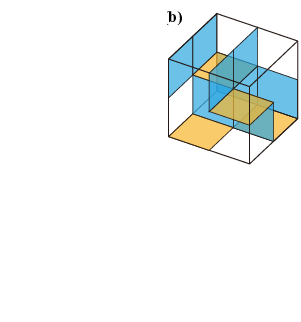
\includegraphics[width=.5\textwidth]{../spspt/blocks}
		\end{center}
		\column{.5\textwidth}
		\begin{center}
			\begin{tikzpicture}
				\draw (-2, -2)--(-2, 2)--(2, 2)--(2, -2)--(-2, -2);
				\draw<2> [thick] (0, -2)--(0, 2);
				\draw [->] (.7, 0) arc (0:180:0.7);
				\filldraw (0, 0) circle (1pt) node [right] {$C_2$};
				\node<2> at (0, -1) [right] {$\tau_1$};
				\node<2> at (0, 1) [left] {$\tau_2$};
				\node<2> at (-1, 0) {$\sigma_1$};
				\node<2> at (1, 0) {$\sigma_2$};
			\end{tikzpicture}
		\end{center}
	\end{columns}
\end{frame}

\begin{frame}
	\frametitle{Topological crystalline states are made of building blocks}
	\begin{columns}
		\column{.4\textwidth}
		\begin{center}
			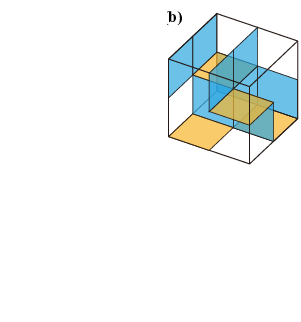
\includegraphics[width=\textwidth]{../spspt/blocks}
		\end{center}
		\column{.6\textwidth}
		\begin{itemize}
			\item We divide the space into cells compatible with the space-group symmetry.
			\item On a $p$-cell $\sigma$, the SPT state is protected only by $G_\sigma$.
			\[\hat\omega(\sigma)\in \Phi^p(G_\sigma) = H^{p+1}[G_\sigma,\uone_T].\]
			\item $G_\sigma$ acts as onsite symmetries.
			\item Decorate 3d SPT on 3-cells; 2d SPT on 2-cells; 1d SPT on 1-cells; 0d SPT on 0-cells;
			\item $p$-block states: $E^p_{p,\infty}$.
			\[\text{TCSs} = ``\bigoplus_p\text{''} E^p_{p,\infty}.\]
		\end{itemize}
	\end{columns}
\end{frame}

%\begin{frame}
%	\frametitle{Symmetric conditions}
%	\begin{columns}
%		\column{.3\textwidth}
%		\begin{tikzpicture}
%			\draw (0, 0)--(2, 0)--(2, 2)--(0, 2)--(0, 0);
%			\draw (2, 4)--(4, 4)--(4, 6)--(2, 6)--(2, 4);
%			\draw [thick,->] (1, 1) node [below] {$\hat\omega(\sigma$)} --
%			(3, 5) node [above] {$\hat\omega(\sigma^\prime)$};
%			\node at (2, 3) [right] {$g$};
%		\end{tikzpicture}
%		\column{.7\textwidth}
%		\begin{itemize}
%			\item If $g:\sigma\rightarrow\sigma^\prime$, then the cochains attached must be ``identical''.
%			\item $G_\sigma\neq G_{\sigma'}$, but they are isomorphic:
%			\[G_{\sigma'}=gG_\sigma g^{-1}\simeq G_\sigma.\]
%			\item This induces another isomorphism:
%			\[H^{p+1}[G_{\sigma'},\uone_T]\simeq H^{p+1}[G_\sigma,\uone_T]\]
%			\item $\hat\omega(\sigma)$ and $\hat\omega(\sigma')$ are related by this isomorphism
%			\[\hat\omega(\sigma') = g\cdot \hat\omega(\sigma).\]
%			\item Only decorations on symmetry-unrelated cells are independent: finite \# of them.
%		\end{itemize}
%	\end{columns}
%\end{frame}

\begin{frame}
	\frametitle{No-Open-Edge Conditions}
	\begin{columns}
		\column{.58\textwidth}
		\begin{itemize}
			\item<1-> SPT blocks have nontrivial boundary states.
			\item<2-> Boundary anomaly must cancel on $(p-1)$-cells.
			\item<3-> $\hat\omega(\sigma_1)
			+\hat\omega(\sigma_2)+\hat\omega(\sigma_3)+\hat\omega(\sigma_4)\simeq0$.
		\end{itemize}
		\column{.42\textwidth}
		\begin{tikzpicture}
			\draw (0, 1)--(-1, 1)--(-2, 0)--(2, 0)--(3, 1)--(1, 1);
			\draw [thick] (0, 0)--(1, 1);
			\draw<1-2> [string] (.2, .1)--(1, .9);
			\draw<1> [string] (1, .9)--(2.8, .9);
			\draw<1> [string] (2.8, .9)--(2, .1);
			\draw<1> [string] (2, .1)--(.2, .1);
			\draw<2> [string] (.1, .2)--(.9, 1);
			\draw<3-> [->] (1.3, .5)--(.6, .5);
			\draw<3-> [->] (.5, 1.3)--(.5, .6);
			\draw<3-> [->] (.5, -.3)--(.5, .4);
			\draw<3-> [->] (-.3, .5)--(.4, .5);
			\node<1-2> at (.5, .5) [above] {$\tau$};
			\node<3-> at (.7, .7) [above] {$\tau$};
			\draw (1, 1)--(1, 3)--(0, 2)--(0, -2)--(0, -2)--(1, -1)--(1, 0);
			\node at (.5, 1.5) {$\sigma_1$};
			\node at (1.5, .5) {$\sigma_2$};
			\node at (.5, -0.5) {$\sigma_3$};
			\node at (-0.5, .5) {$\sigma_4$};
		\end{tikzpicture}
	\end{columns}
\end{frame}

\begin{frame}
	\frametitle{Bubbling Equivalence}
\begin{columns}
\column{.7\textwidth}
\begin{itemize}
\item A bubbling process: fill a 2-cell with a loop of 1-dim SPT states.
\item Changes 1-cell decoration.
\item Does not change bulk classification.
\item Two decorations should be viewed as equivalent ones.
\end{itemize}
\column{.3\textwidth}
\begin{animateinline}{5}
        \multiframe{12}{Ra=.3+.05}{
\begin{tikzpicture}[scale=1]
	\draw (0, 0)--(2, 0)--(2, 2)--(0, 2)--(0, 0);
	\draw [dashed] (1, 2)--(1, 1)--(2, 1);
	\draw (2, 1)--(3, 1)--(3, 3)--(1, 3)--(1, 2);
	\draw [dashed] (0, 0)--(1, 1);
	\draw (2, 0)--(3, 1);
	\draw (0, 2)--(1, 3);
	\draw (2, 2)--(3, 3);
	\fill [blue!30,opacity=.5] (1.5-1.5*\Ra, 1.5-1.5*\Ra)--(1.5+0.5*\Ra, 1.5-1.5*\Ra)
	--(1.5+1.5*\Ra, 1.5-0.5*\Ra)--(1.5+1.5*\Ra, 1.5+1.5*\Ra)
	--(1.5-0.5*\Ra, 1.5+1.5*\Ra)--(1.5-1.5*\Ra, 1.5+0.5*\Ra)
	--(1.5-1.5*\Ra, 1.5-1.5*\Ra);
	\draw [blue,dashed] (1.5-1.5*\Ra, 1.5+0.5*\Ra)--(1.5+0.5*\Ra, 1.5+0.5*\Ra)--(1.5+1.5*\Ra,1.5+1.5*\Ra);
	\draw [blue,dashed] (1.5+0.5*\Ra, 1.5-1.5*\Ra)--(1.5+0.5*\Ra, 1.5+0.5*\Ra);
	\draw [->,thick] (1.5-0.5*\Ra, 1.5-0.5*\Ra)--(1.3-0.5*\Ra, 1.3-0.5*\Ra);
	\draw [->,thick] (1.5, 1.5+\Ra)--(1.5, 1.78+\Ra);
	\draw [->,thick] (1.5+\Ra, 1.5)--(1.78+\Ra, 1.5);
	%\fill [green!30] (-\Ra,-\Ra)--(-\Ra,\Ra)--(\Ra,\Ra)--(\Ra,-\Ra)--(-\Ra,-\Ra);
%\draw [blue,thick] (-\Ra,-\Ra)--(-\Ra,\Ra)--(\Ra,\Ra)--(\Ra,-\Ra)--(-\Ra,-\Ra);
%\node at (0, 0) {$d\nu$};
\end{tikzpicture}
}
\end{animateinline}
\end{columns}
\end{frame}

\begin{frame}
\frametitle{High-Order No-Open-Edge Conditions}
\begin{columns}
\column{.6\textwidth}
\begin{enumerate}
\item<1-> Choose a cocycle for each 2-cell $\sigma$.\\ Check $\partial\hat\omega_2(\tau)\simeq0$ for each 1-cell $\tau$.\\
\emph{1st-page no-open-edge condition.}
\item<2-> Choose a cochain $\hat\omega_1$ for each $\tau$.\\
Check $\partial\hat\omega_1(\lambda)\simeq0$ for each 0-cell $\lambda$.\\
\emph{2nd-page no-open-edge condition.}
\item<3> Choose a cochain $\hat\omega_0$ for each $\lambda$.
\end{enumerate}
\column{.4\textwidth}
\begin{center}
\begin{tikzpicture} [scale=3]
\fill [blue!50] (0,0)--(1,0)--(1.5,.5)--(1.5,1.5)--(0.5,1.5)--(0,1)--(0,0);
\draw<1> [thick,white] (0,0)--(1,0)--(1,1)--(0,1)--(0,0);
\draw<1> [thick,white] (1,0)--(1.5,.5)--(1.5,1.5)--(1,1);
\draw<1> [thick,white] (1.5,1.5)--(0.5,1.5)--(0,1);
\draw<1> [thick,white] (0,0)--(.5,.5)--(.5,1.5);
\draw<1> [thick,white](.5,.5)--(1.5,.5);
\draw<2-> [thick,red] (0,0)--(1,0)--(1,1)--(0,1)--(0,0);
\draw<2-> [thick,red] (1,0)--(1.5,.5)--(1.5,1.5)--(1,1);
\draw<2-> [thick,red] (1.5,1.5)--(0.5,1.5)--(0,1);
\draw<2-> [thick,red] (0,0)--(.5,.5)--(.5,1.5);
\draw<2-> [thick,red](.5,.5)--(1.5,.5);
\fill<1-2> [white] (0,0) circle (2pt);
\fill<1-2> [white] (1,0) circle (2pt);
\fill<1-2> [white] (0,1) circle (2pt);
\fill<1-2> [white] (1,1) circle (2pt);
\fill<1-2> [white] (0.5,0.5) circle (2pt);
\fill<1-2> [white] (1.5,0.5) circle (2pt);
\fill<1-2> [white] (0.5,1.5) circle (2pt);
\fill<1-2> [white] (1.5,1.5) circle (2pt);
\fill<3> [red] (0,0) circle (2pt);
\fill<3> [red] (1,0) circle (2pt);
\fill<3> [red] (0,1) circle (2pt);
\fill<3> [red] (1,1) circle (2pt);
\fill<3> [red] (0.5,0.5) circle (2pt);
\fill<3> [red] (1.5,0.5) circle (2pt);
\fill<3> [red] (0.5,1.5) circle (2pt);
\fill<3> [red] (1.5,1.5) circle (2pt);
\end{tikzpicture}
\end{center}
\end{columns}
\end{frame}

\begin{frame}
\frametitle{High-Order Bubbling Equivalences}
\begin{itemize}
\item Similarly, there are high-order bubbling equivalence.
\item Assign 1d SPT states ($d\hat\mu_1=0$) to 2-cells: $\partial\hat\mu_2$ trivializes $\hat\omega_1$ building blocks.
\item If $\partial\hat\mu_2\simeq0$, choose $d\hat\mu_1+\partial\hat\mu_2=0$, then $\partial\hat\mu_1$ trivializes $\hat\omega_0$ building blocks.
\item High-order computations are organized as a \alert{spectral sequence}.
\end{itemize}
\begin{center}
\begin{animateinline}{5}
        \multiframe{12}{Ra=.4+.05}{
\begin{tikzpicture}
	\draw (-2,-2)--(-2,2)--(2,2)--(2,-2)--(-2,-2);
   \draw (-2,0)--(2,0);
   \draw (0,-2)--(0,2);
	%\fill [green!30] (-\Ra,-\Ra)--(-\Ra,\Ra)--(\Ra,\Ra)--(\Ra,-\Ra)--(-\Ra,-\Ra);
\draw [blue,thick] (-\Ra+1,-\Ra+1)--(-\Ra+1,\Ra+1)--(\Ra+1,\Ra+1)--(\Ra+1,-\Ra+1)--(-\Ra+1,-\Ra+1);
\draw [blue,thick] (-\Ra+1,-\Ra-1)--(-\Ra+1,\Ra-1)--(\Ra+1,\Ra-1)--(\Ra+1,-\Ra-1)--(-\Ra+1,-\Ra-1);
\draw [blue,thick] (-\Ra-1,-\Ra+1)--(-\Ra-1,\Ra+1)--(\Ra-1,\Ra+1)--(\Ra-1,-\Ra+1)--(-\Ra-1,-\Ra+1);
\draw [blue,thick] (-\Ra-1,-\Ra-1)--(-\Ra-1,\Ra-1)--(\Ra-1,\Ra-1)--(\Ra-1,-\Ra-1)--(-\Ra-1,-\Ra-1);
%\node at (0, 0) {$d\nu$};
%\node at (\Ra, 0) [left] {$\nu$};
\end{tikzpicture}
}
\end{animateinline}
~~~~
\begin{animateinline}{5}
        \multiframe{8}{Ra=.8+-.1}{
\begin{tikzpicture}
\draw (-2,0)--(2,0);
\draw (0, -2)--(0, 2);
\draw [blue,thick,double] (-\Ra, 0)--(\Ra,0);
\draw [blue,thick,double] (2-\Ra,0)--(2,0);
\draw [blue,thick,double] (-2+\Ra,0)--(-2,0);
\draw [blue,thick,double] (0, -\Ra)--(0, \Ra);
\draw [blue,thick,double] (0, 2-\Ra)--(0, 2);
\draw [blue,thick,double] (0, -2+\Ra)--(0, -2);
\fill [red] (-\Ra,0) circle (2pt);
\fill [red] (\Ra,0) circle (2pt);
\fill [red] (0,-\Ra) circle (2pt);
\fill [red] (0,\Ra) circle (2pt);
\fill [red] (2-\Ra,0) circle (2pt);
\fill [red] (-2+\Ra,0) circle (2pt);
\fill [red] (0,2-\Ra) circle (2pt);
\fill [red] (0,-2+\Ra) circle (2pt);
\end{tikzpicture}
}
\end{animateinline}
\end{center}
\end{frame}

\begin{frame}
\frametitle{Mathematical Proof for bosonic SPTs}
\begin{itemize}
\item Equivariant group cohomology:
\[H^{d+1}[G, \uone_{PT}]]\simeq H^{d+1}_G[X, \uone_{PT}].\]
Here $X\sim\text{pt}$ is a (non-free) $G$-complex. See Thorngren and Else, PRX (2018).
\item There is a spectral sequence:
\[E_1^{pq}=\bigoplus_{\sigma\in X_p/G}H^q[G_\sigma,\uone_T]\Rightarrow
 H^{p+q}[G, \uone_{PT}]].\]
See Kenneth S. Brown's book, Chapter VII.
\item The topological space $Y$ we used is the Poincar\'e dual of $X$: $E^{pq}_r\simeq E^{q-1}_{d-p,r}$
\end{itemize}
\begin{center}
	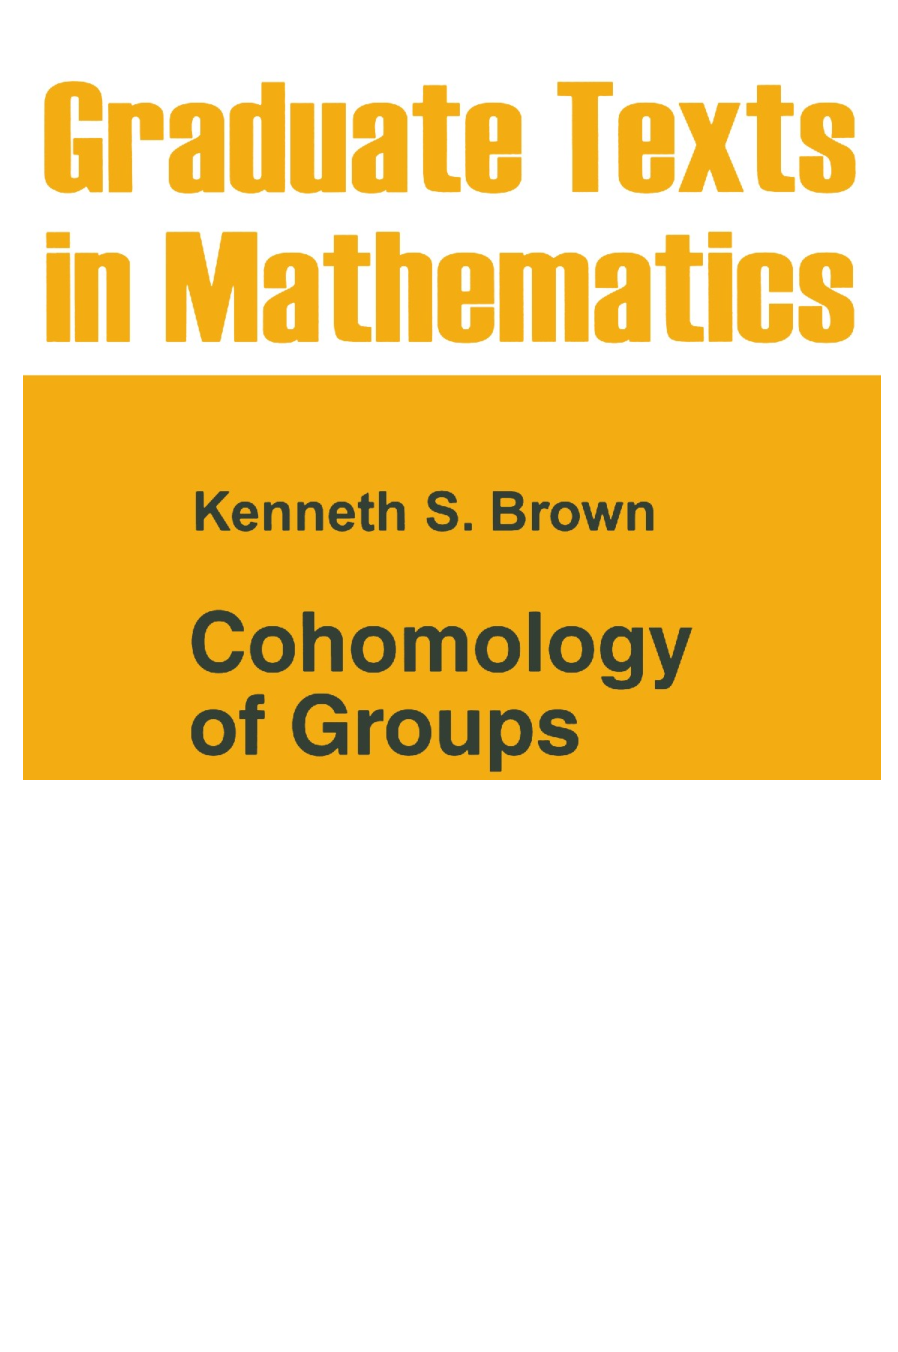
\includegraphics[height=2cm]{brown_book}
	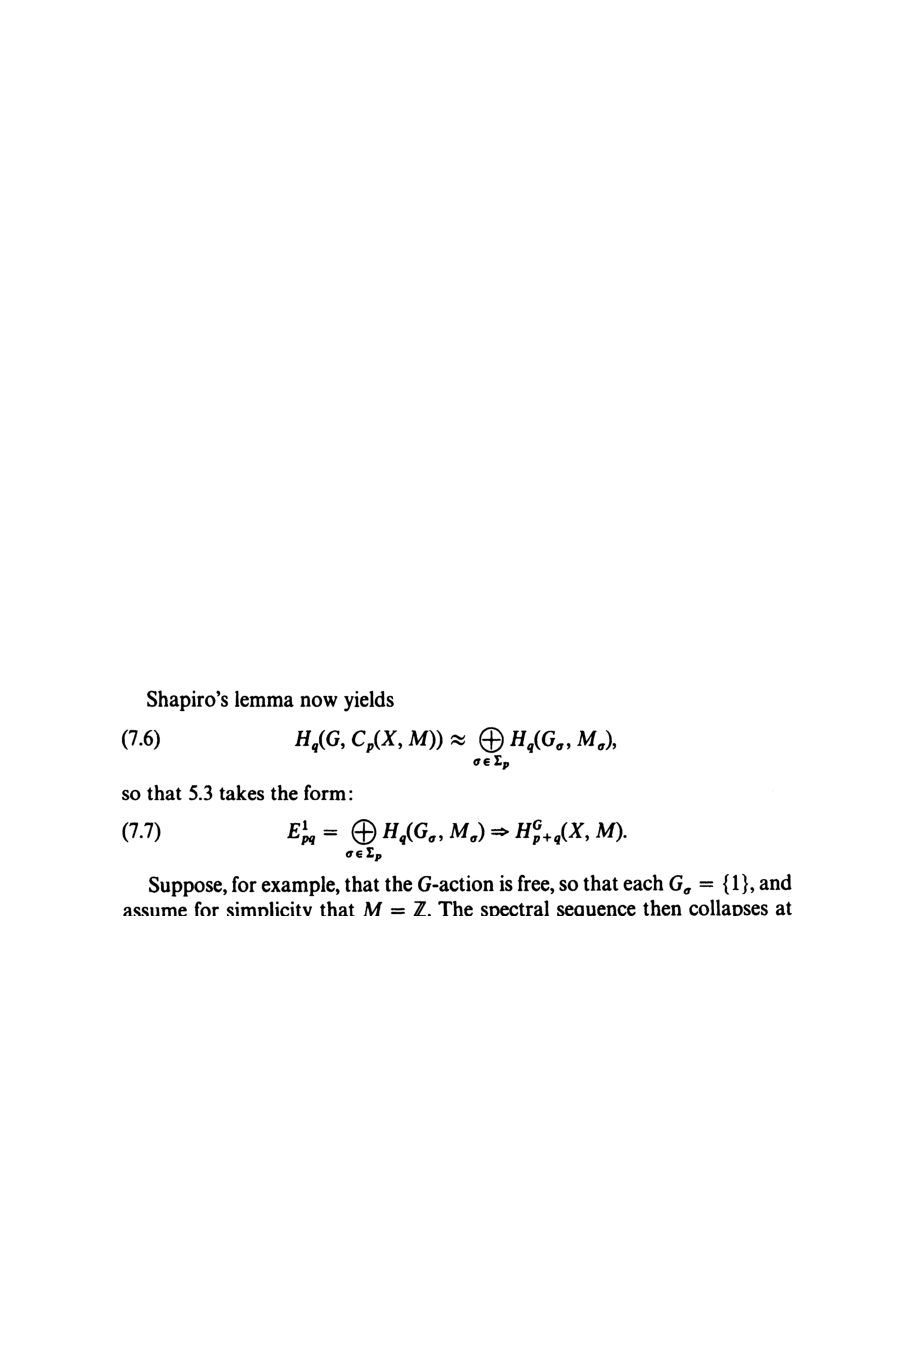
\includegraphics[height=2cm]{brown_ss}
\end{center}
\end{frame}

\begin{frame}
  \frametitle{Real-space construction of fSPTs}

  \begin{itemize}
  \item Interacting fSPTs:
    \begin{itemize}
    \item 2D point groups: Jian-Hao Zhang, Qing-Rui Wang, Shuo Yang, YQ and Zheng-Cheng Gu,
      PRB \textbf{101}, 100501(R) (2020).
    \item 2D wallpaper groups: Jian-Hao Zhang, Shuo Yang, YQ and Zheng-Cheng Gu,
      PR Research \textbf{4}, 033081 (2022).
    \item 3D point groups: Jian-Hao Zhang, YQ and Zheng-Cheng Gu, arXiv:2204.13558.
    \end{itemize}
  \item Free-fermion high-order states:
    Tian Yuan, Chen Fang and YQ, to appear.
  \end{itemize}
  \begin{center}
    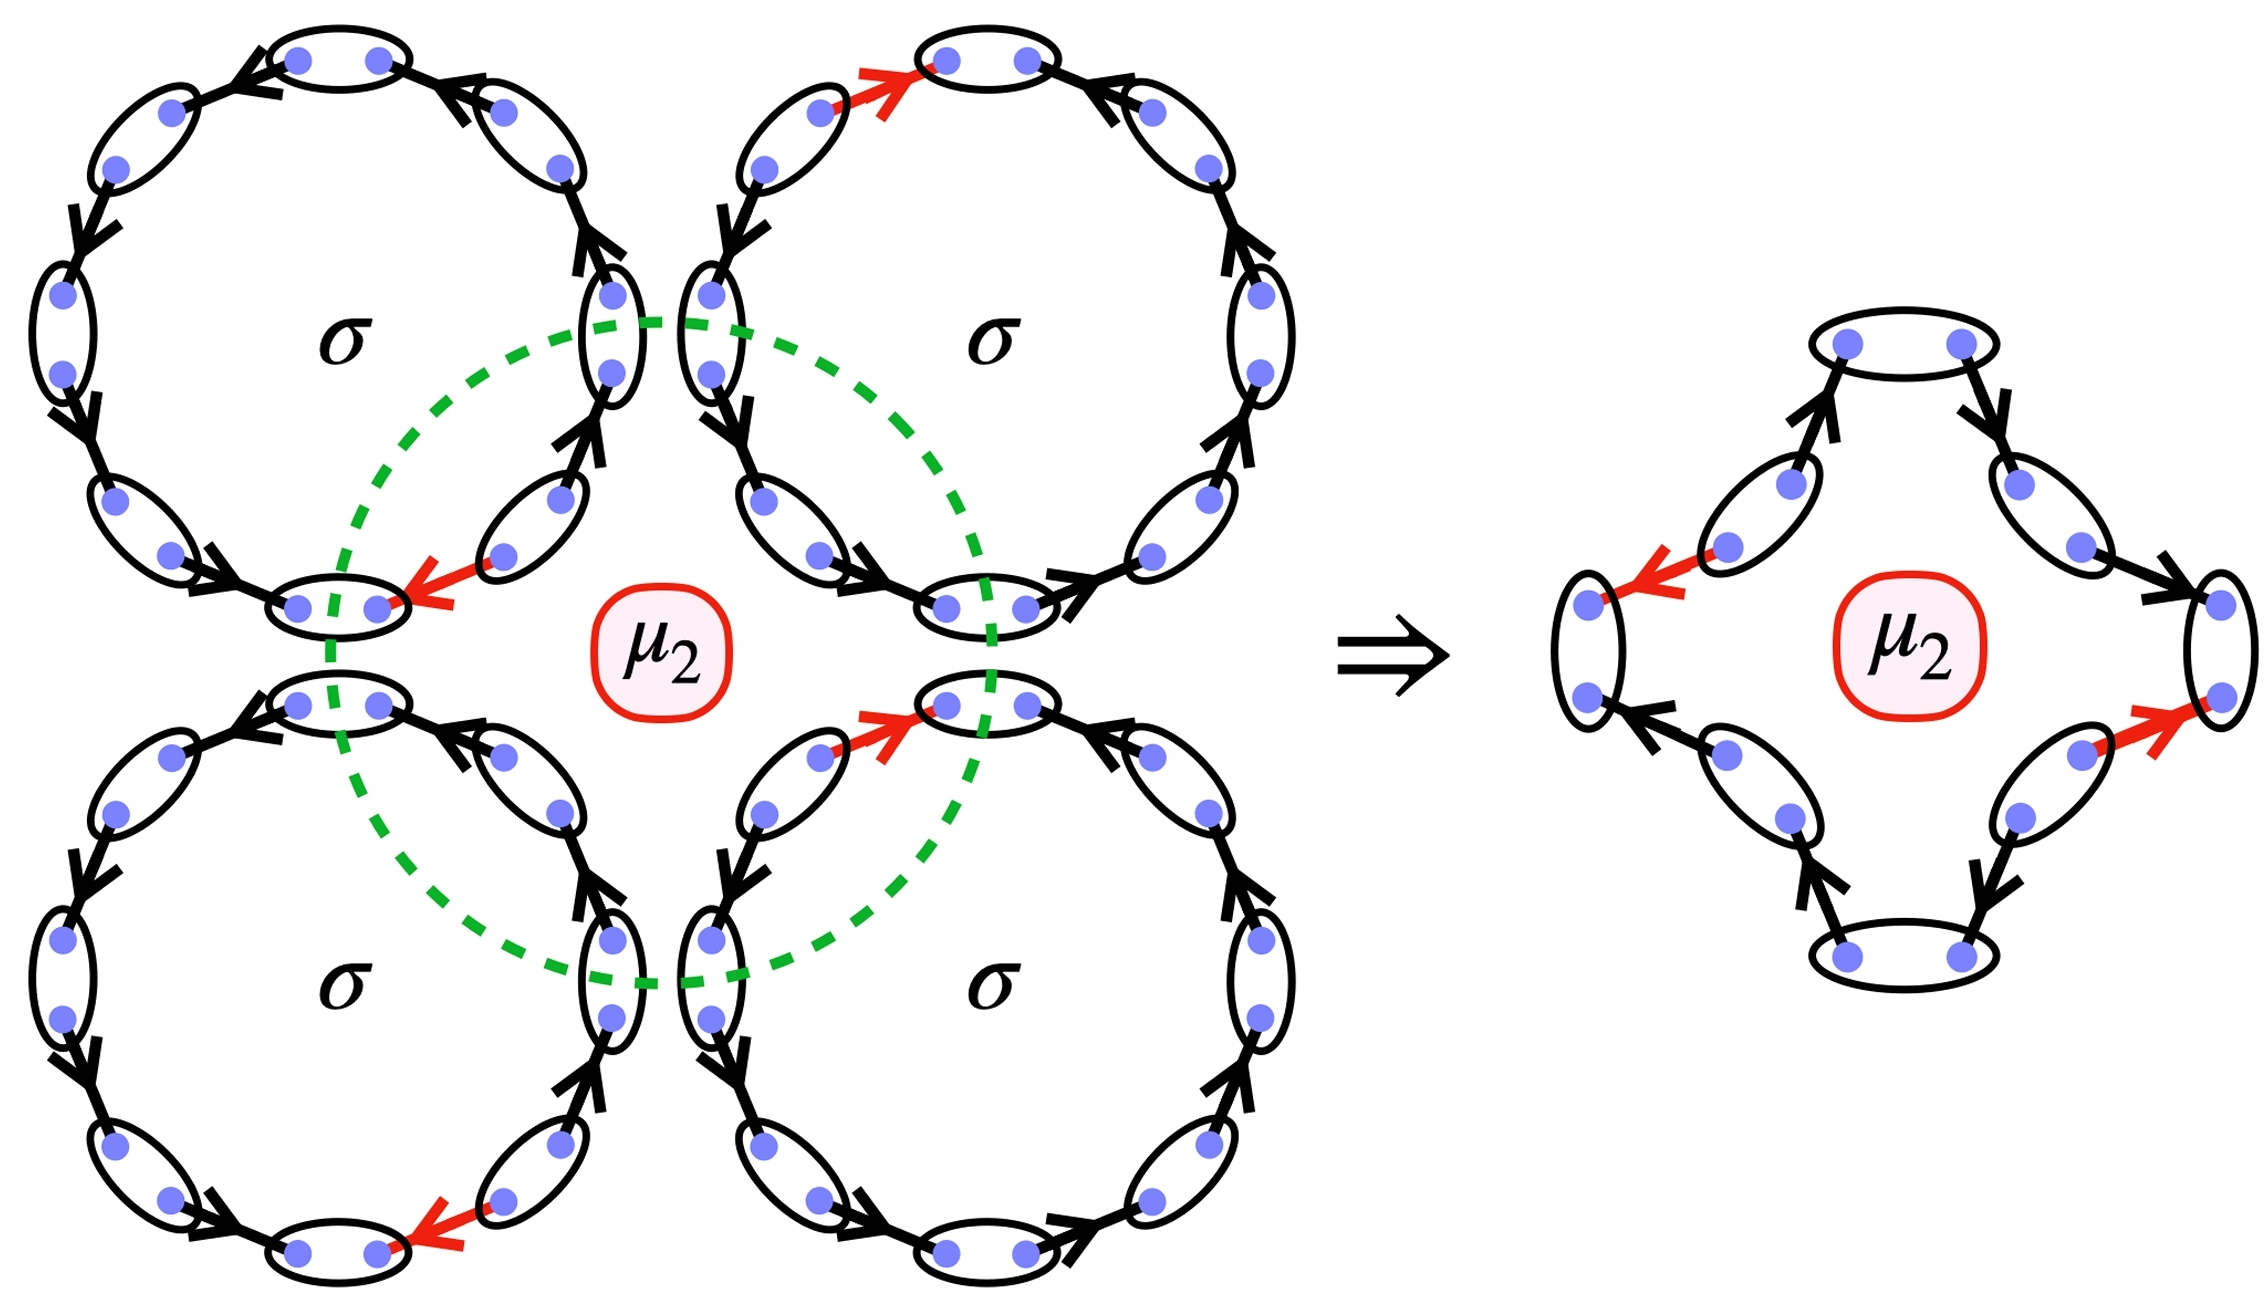
\includegraphics[height=4cm]{majorana_bubble}    
  \end{center}
\end{frame}

\section{Approach II: use crystalline equivalence principle}

\begin{frame}
  \frametitle{Crystalline equivalence principle}
  \begin{itemize}
  \item SPT classification remains the same, if:
    \begin{enumerate}
    \item Crystalline symmetry group $\Rightarrow$ onsite symmetry group.\\
      \emph{Example: $C_2$-SPT = $\mathbb Z_2$-SPT.}
    \item Symmetries reversing space orientation $\Rightarrow$ antiunitary symmetries.\\
      \emph{Example: mirror reflection, glide phane, ...}
    \item For fermions: spinless/spin-$\frac12$ $\Rightarrow$ spin-$\frac12$/spinless.\\
      \emph{Example: $C_2^2=\pm1 \Rightarrow g^2=\mp1$.}
    \end{enumerate}
  \item We can compute crystalline-SPT as onsite-SPTs.
  \item Large symmetry groups (space groups are infinite): need an efficient algorithm.
  \end{itemize}
  \begin{center}
    \begin{tikzpicture}
      \draw (-6, -1.5)--(-6, 1.5)--(-3, 1.5)--(-3, -1.5)--(-6, -1.5);
    \draw [->] (-5, .3)--(-5, .7);
    \draw [->] (-4, .3)--(-4, .7);
    \draw [->] (-5, -.3)--(-5, -.7);
    \draw [->] (-4, -.7)--(-4, -.3);
    \node at (-2.25, 0) {=};

    \draw (-1.5, -1.5)--(-1.5, 1.5)--(1.5, 1.5)--(1.5, -1.5)--(-1.5, -1.5);
    \draw [->] (.7, 0) arc (0:180:0.7);
    \filldraw (0, 0) circle (1pt) node [right] {$C_2$};
\end{tikzpicture}    
  \end{center}
\end{frame}

\begin{frame}{SptSet: A GAP package for computing SPT classifications}
  \begin{itemize}
  \item SPT classification: generalized cohomology theory of symmetry group $G$.
  \item Atiyah–Hirzebruch Spectral Sequence: SPT of interacting fermions are described by combinations of cochains:
    \[n_1(g_1); n_2(g_1, g_2); \nu_3(g_1,g_2,g_3).\]
  \item A computational challenge:
    \begin{itemize}
    \item Complexity: $O(N^3)$;
    \item Traditionally: $N=(|G|-1)^{d+1}$; very expensive if $d$ and $G$ is large.
    \end{itemize}
  \item Our method:
    \begin{enumerate}
    \item Choose a different \alert{resolution} such that $N$ is small. ($N<100$ for all space groups.)
    \item Use chain maps to translate obstruction functions to new resolution.
    \end{enumerate}
  \item GAP = Group, Algorithm and Programming.
  \item SptSet: A GAP package.
  \end{itemize}
\end{frame}



\begin{frame}[fragile]{Example: fSPT for 2D wallpaper groups}
	\url{SptSet/examples/fspt_2d_s12.g}
	\begin{lstlisting}[basicstyle=\footnotesize]
    for it in [2..17] do
      SG := SpaceGroupBBNWZ(2, it);
      fSG := IsomorphismPcpGroup(SG);
      SG1 := Image(fSG);
      R := ResolutionAlmostCrystalGroup(SG1, 6);
      gs := GeneratorsOfGroup(SG);
      w := Spin12Factor(2, it);
      ww := {g1, g2} -> w(PreImageElm(fSG, g1), PreImageElm(fSG, g2));
      f := GroupHomomorphismByImagesNC(SG1, GL(1, Integers),
        List(gs, x -> Image(fSG, x)),
        List(gs, x -> [[DeterminantMat(x)]]));

      SS := FermionSPTSpecSeq(R, f, ww);
      FermionSPTLayersVerbose(SS, 2);
    od;
  \end{lstlisting}
  17 wallpaper groups in ~6 minutes.
\end{frame}

\section{Conclusion}

\begin{frame}
\frametitle{Summary: towards a complete classification of TCS}
\begin{itemize}
\item Crystalline symmetry: treat as onsite symmetry / real-space construction.
\item Real-space construction
  \begin{itemize}
  \item General rules are known.
  \item Many examples are studied.
  \item Automated computation for interacting-fermion systems?
  \end{itemize}
\item Treat as onsite symmetry:
  \begin{itemize}
  \item 1D \ding{51}, 2D \ding{51}, 3D ??
  \item SptSet package: work in progress.
  \end{itemize}
\item Crosschecked results using the crystalline equivalence principle.
\end{itemize}
\end{frame}

\end{document}
